% -------------------------------------------------------
%  Section 5: Dataset & preprocessing
% -------------------------------------------------------
\section{مجموعه‌داده و پیش‌پردازش}
\label{sec:dataset}

ارزیابی تنها روی \lr{Microsoft Malware Classification Challenge} \cite{ronen2018big2015} انجام شده است: \num{۱۰٬۸۶۸} نمونه آموزش برچسب‌دار و \num{۱۰٬۸۷۳} نمونه آزمون بدون برچسب از ۹ خانواده. هر نمونه یک فایل \kd{.bytes} (محتوای دودویی) و یک فایل \kd{.asm} (خروجی دیس‌اسمبلر \lr{IDA}) دارد. توزیع کلاس‌ها به‌شدت نامتوازن است، از \num{۲٬۹۴۲} نمونه برای \lr{Kelihos\_ver3} تا تنها \num{۴۲} نمونه برای \lr{Simda}؛ مقاله این را گزارش می‌کند ولی هیچ تدبیری برای آن نمی‌اندیشد و هیچ سنجه متوازنی ارائه نمی‌دهد.

\subsection{یک وابستگی مهم که کم‌رنگ مانده است}
فایل‌های \kd{.bytes} به‌دلایل امنیتی فاقد \lr{PE-Header} هستند، پس جدول بخش‌ها را نمی‌توان از آن‌ها استخراج کرد؛ مقاله این مشکل را با خواندن نشانگر‌های ابتدای هر بخش از فایل \kd{.asm} حل می‌کند. پیامد آن است که خط لوله پیشنهادی، برخلاف آنچه چارچوب‌بندی مقاله القا می‌کند، \textbf{صرفاً بایت‌محور نیست} و به خروجی یک دیس‌اسمبلر تجاری وابسته است. این نکته از آن جهت اهمیت دارد که مقاله در بخش کارهای مرتبط، دقیقاً پرهیز از دیس‌اسمبل را به‌عنوان مزیت خانواده روش‌های مصورسازی برمی‌شمارد؛ یعنی روش پیشنهادی بخشی از همان هزینه‌ای را بازمی‌گرداند که مصورسازی قرار بود حذف کند و در برابر همان مبهم‌سازی‌هایی آسیب‌پذیر می‌شود که تحلیل ایستا را هدف می‌گیرند. مقاله این وابستگی را پنهان نمی‌کند، اما آن را به‌عنوان محدودیت هم صورت‌بندی نمی‌کند. به همین دلیل، رده \lr{HEADER} نیز برای این مجموعه‌داده بی‌اثر است و جدول ۱ مقاله در عمل تنها برای چهار بخش به کار می‌آید.

\subsection{پیش‌پردازش}
بایت‌های ناشناخته (\kd{??}) به‌جای حذف، یکنواخت به صفر نگاشته می‌شوند؛ انتخاب ساده و قابل دفاعی است، هرچند این پیکسل‌های صفر با پیکسل‌های صفر ناشی از هم‌ترازی فایل تمیزناپذیر می‌شوند. در \lr{S4} و \lr{S5} عرض پایه پیش از قطعه‌بندی روی \num{۱۰۲۴} ثابت می‌شود تا اثر عرض از اثر قطعه‌بندی جدا بماند؛ تصمیم روش‌شناختی درستی است. شکل \ref{fig:paperwidth} نشان می‌دهد که چرا عرض اصلاً اهمیت دارد: یک نمونه واحد زیر سه طرح هم‌ترازی، سه بافت کاملاً متفاوت تولید می‌کند.

\begin{figure}[!ht]
    \centering
    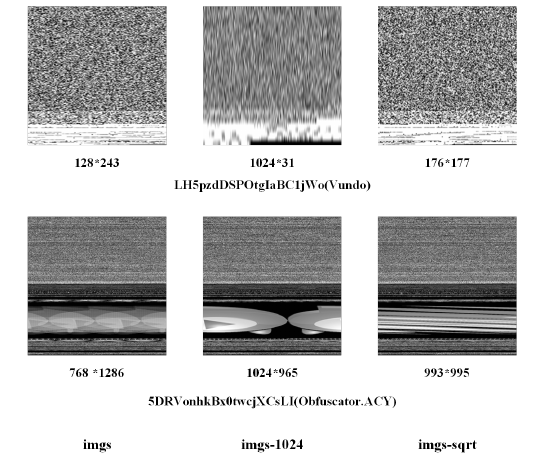
\includegraphics[width=0.37\textwidth]{figs/paper_width.png}
    \caption{اثر طرح هم‌ترازی عرض بر تصویر خاکستری، از شکل ۴ مقاله. هر ردیف یک نمونه واحد است که با سه طرح \lr{S1}، \lr{S3} و \lr{S2} رستر شده است.}
    \label{fig:paperwidth}
\end{figure}

نکته‌ای که مقاله درباره آن سکوت می‌کند، سرنوشت نمونه‌هایی است که یک بخش خاص را ندارند؛ در پیکربندی‌های چندکاناله باید کانال متناظر با چیزی پر شود و متن این حالت را پوشش نمی‌دهد. در بازپیاده‌سازی خودمان (\S\ref{sec:repro}) این حالت را با تولید یک کانال تمام‌صفر در زمان پیش‌پردازش مدیریت کردیم؛ انتخابی که ناگزیر بود ولی خودسرانه است و یکی از نقاطی است که بازتولید بیت‌به‌بیت مقاله را ناممکن می‌سازد.
